
\subsection{Literature Overview}
The study of ladder lottieres as mathematical objects began in 2010, in  the paper
\textbf{Efficient Enumeration of Ladder Lotteries and its Application}. The paper was 
written by four authors, Yamanaka, Horiyama, Uno and Wasa. In this paper the 
authors present an algorithm for generating all the ladder lotteries of an 
arbitrary permutation, $\pi$. Since this paper emerged, there have been 
several other paper written directly about ladder lotteries. 
These papers include \textbf{The Ladder Lottery Realization Problem},
\textbf{Optimal Reconfiguration of Optimal Ladder Lotteries}, 
\textbf{Efficient Enumeration of all Ladder Lotteries with K Bars},
\textbf{Coding Ladder Lotteries} and
\textbf{Enumeration, Counting, and Random Generation of Ladder Lotteries}.
\section{Efficient Enumeration of Ladder Lotteries and its Application}

%%Intro
In the Efficient Enumeration of Ladder Lotteries and its Application, written by Matsui, Nakada, Nakano Uehara and Yamanaka,
the authors provide an algorithm for generating $OptL\{\pi\}$ 
for any $\pi$, in $\mathcal{O}(1)$ per ladder~\cite{A1}. The authors refer to this algorithm as {\sc FindAllChildren}
which can be found in Algorithm~\ref{Alg:FindAllChildren}. 
\begin{algorithm}[!htp]
	\begin{algorithmic}[1]
		\Function{FindAllChildren}{$ladder$, $cleanLevel$, $n$}
			\State $currentRoute \gets n$
			\While{$currentRoute \geq cleanLevel$}
				\State going top left to bottom right 
				\For{$bar \in currentRoute$}
					\State $row \gets$ row of $bar$ in $ladder$ 
					\State $col \gets$ col of $bar$ in $ladder$
					\State $lowerNeighbor \gets ladder[row-1][col]$
					\If{$lowerNeighbor$ is right swappable}
						\State {\sc RightSwap($ladder$, $bar$, $lowerNeighbor$)}
						\State {\sc {\sc FindAllChildren}($ladder$, $y+1$, $n$)}
						\State {\sc LeftSwap($ladder$, $bar$, $lowerNeighbor$)}
					\EndIf
				\EndFor
				\State $currentRoute \gets currentRoute-1$
			\EndWhile
			\State $currentRoute \gets cleanLevel-1$
			\For{$bar \in currentRoute$}
				\State $row \gets$ row of $bar$ in $ladder$ 
				\State $col \gets$ col of $bar$ in $ladder$
				\State $lowerNeighbor \gets ladder[row-1][col]$
				\If{$lowerNeighbor$ is right swappable \textbf{and} is the rightmost bar of $currentRoute-1$}
					\State {\sc RightSwap($ladder$, $bar$)}
					\State {\sc FindAllChildren($ladder$, $cleanLevel$, $n$)}
					\State {\sc LeftSwap($ladder$, $bar$)}
				\EndIf
			\EndFor
		\EndFunction
	\end{algorithmic}
	\caption{The algorithm for listing $OptL\{\pi\}$.}
	\label{Alg:FindAllChildren}
\end{algorithm}
\pagebreak

One will note that two helper functions, {\sc RightSwap} and {\sc LeftSwap}, are required to complete 
{\sc FindAllChildren}. The details of these algorithms are not found 
in the paper~\cite{A1}. Thus, these algorithms and their details can be found in the Appendix in Algorithm \ref{Alg:RightSwap}
and Algorithm \ref{Alg:LeftSwap}.
{\sc FindAllChildren} is the first algorithm for generating $OptL\{\pi\}$.\newline
{\sc FindAllChildren} enumerates $OptL\{\pi\}$ as a tree of ladders.

%%Put this in the Appendix

%%DONE PUT IN Appendix

%%%%%%%%%%%%%%%%%%%%%%%%%%%%%%%FIND ALL CHILDREN ALGORITHM%%%%%%%%%%%%%%%%%%%%%%%%%%%%%



%%%%%%%%%%%%%%%%%%END ALGORITHM%%%%%%%%%%%%%%%%%%%%%%%%%%



{\sc FindAllChildren} was used in this thesis to generate the sample data that aided in finding solutions for 
the Gray Code Problem in Chapter 3 and the Minimum Height Problem in Chapter 4.  
Therefore, this algorithm is paramount for the findings of this thesis. 
To see the tree structure generated by {\sc FindAllChildren} for $OptL\{(4,3,2,1)\}$ 
please refer to Figure~\ref{Fig:TreeFAC}. 
\begin{figure}[h]
	\centering 
	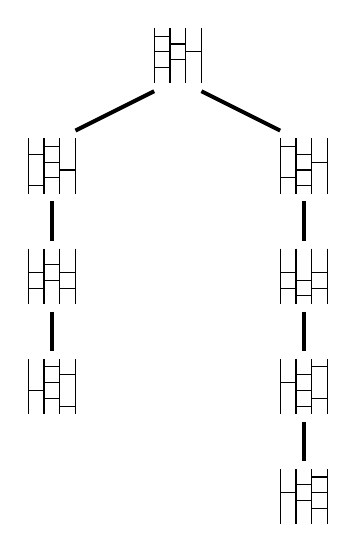
\begin{tikzpicture}
		%%L1
		\draw(5, 10) to (5, 9.3);
			\draw(5, 9.9) to (5.2, 9.9);
			\draw(5.2, 9.8) to (5.4, 9.8);
			\draw(5.4, 9.7) to (5.6, 9.7);
		\draw(5.2, 10) to (5.2, 9.3);
			\draw(5, 9.7) to (5.2, 9.7);
			\draw(5.2, 9.6) to (5.4, 9.6);
		\draw(5.4, 10) to (5.4, 9.3);
			\draw(5, 9.5) to (5.2, 9.5);
		\draw(5.6, 10) to (5.6, 9.3);
		%L2
		\draw[line width = .5mm](5, 9.2) to (4, 8.7);
		\draw[line width = .5mm](5.6, 9.2) to (6.6, 8.7);
			%%L2
			\draw(3.4, 8.6) to (3.4, 7.9);
				\draw(3.4, 8.4) to (3.6, 8.4);
				\draw(3.4, 8) to (3.6, 8);
			\draw(3.6, 8.6) to (3.6, 7.9);
				\draw(3.6, 8.5) to (3.8, 8.5);
				\draw(3.6, 8.3) to (3.8, 8.3);
				\draw(3.6, 8.1) to (3.8, 8.1);
			\draw(3.8, 8.6) to (3.8, 7.9);
				\draw(3.8, 8.2) to (4, 8.2);
			\draw(4.0, 8.6) to (4.0, 7.9);

				%%level
				\draw[line width = .5mm](3.7, 7.8) to (3.7, 7.3);
			\draw(3.4, 7.2) to (3.4, 6.5);
				\draw(3.4, 6.9) to (3.6, 6.9);
				\draw(3.4, 6.7) to (3.6, 6.7);
			\draw(3.6, 7.2) to (3.6, 6.5);
				\draw(3.6, 7) to (3.8, 7);
				\draw(3.6, 6.8) to (3.8, 6.8);
			\draw(3.8, 7.2) to (3.8, 6.5);
				\draw(3.8, 6.9) to (4, 6.9);
				\draw(3.8, 6.7) to (4, 6.7);
			\draw(4.0, 7.2) to (4.0, 6.5);

		%%L3
			\draw(6.6, 8.6) to (6.6, 7.9);
				\draw(6.6, 8.5) to (6.8, 8.5);
				\draw(6.8, 8.4) to (7, 8.4);
				\draw(7, 8.3) to (7.2, 8.3);
			\draw(6.8, 8.6) to (6.8, 7.9);
				\draw(6.8, 8.2) to (7, 8.2);
				\draw(6.8, 8) to (7, 8);
			\draw(7, 8.6) to (7, 7.9);
				\draw(6.6, 8.1) to (6.8, 8.1);
			\draw(7.2, 8.6) to (7.2, 7.9);
			
			
			\draw[line width = .5mm](6.9, 7.8) to (6.9, 7.3);

			\draw(6.6, 7.2) to (6.6, 6.5);
				\draw(6.6, 6.9) to (6.8, 6.9);
				\draw(6.6, 6.7) to (6.8, 6.7);
			\draw(6.8, 7.2) to (6.8, 6.5);
				\draw(6.8, 6.8) to (7, 6.8);
				\draw(6.8, 6.6) to (7, 6.6);
			\draw(7.0, 7.2) to (7.0, 6.5);
				\draw(7, 6.9) to (7.2, 6.9);
				\draw(7, 6.7) to (7.2, 6.7);
			\draw(7.2, 7.2) to (7.2, 6.5);

			\draw[line width = .5mm](3.7, 6.4) to (3.7, 5.9);

			\draw(3.4, 5.8) to (3.4, 5.1);
				\draw(3.4, 5.4) to (3.6, 5.4);
			\draw(3.6, 5.8) to (3.6, 5.1);
				\draw(3.6, 5.7) to (3.8, 5.7);

				\draw(3.6, 5.5) to (3.8, 5.5);
				\draw(3.6, 5.3) to (3.8, 5.3);
			\draw(3.8, 5.8) to (3.8, 5.1);
				\draw(3.8, 5.6) to (4, 5.6);
				\draw(3.8, 5.2) to (4, 5.2);
			\draw(4.0, 5.8) to (4.0, 5.1);

			\draw[line width = .5mm](6.9, 6.4) to (6.9, 5.9);

			
			\draw(6.6, 5.8) to (6.6, 5.1);
				\draw(6.6, 5.5) to (6.8, 5.5);
			\draw(6.8, 5.8) to (6.8, 5.1);
				\draw(6.8, 5.6) to (7, 5.6);

				\draw(6.8, 5.4) to (7, 5.4);
				\draw(6.8, 5.2) to (7, 5.2);
			\draw(7.0, 5.8) to (7.0, 5.1);
				\draw(7.0, 5.7) to (7.2, 5.7);
				\draw(7.0, 5.3) to (7.2, 5.3);
			\draw(7.2, 5.8) to (7.2, 5.1);

			\draw[line width = .5mm](6.9, 5) to (6.9, 4.5);

			\draw(6.6, 4.4) to (6.6, 3.7);
				\draw(6.6, 4.1) to (6.8, 4.1);
			\draw(6.8, 4.4) to (6.8, 3.7);
				\draw(6.8, 4.2) to (7, 4.2);

				\draw(6.8, 4) to (7, 4);
			\draw(7.0, 4.4) to (7.0, 3.7);
				\draw(7.0, 4.3) to (7.2, 4.3);
				\draw(7.0, 4.1) to (7.2, 4.1);
				\draw(7.0, 3.9) to (7.2, 3.9);
			\draw(7.2, 4.4) to (7.2, 3.7);



	\end{tikzpicture}
	\caption{The tree structure of $OptL\{(4,3,2,1)\}$ generated by {\sc FindAllChildren}}
	\label{Fig:TreeFAC}
\end{figure}
\pagebreak
{\sc FindAllChildren} is based on several key concepts. One of which is the local swap operation 
which has already been discussed. The next fundamental concept is the \emph{route} of an element, 
which is the sequence of bars the element travels along in order to reach its final position in the 
sorted permutation. The bars are read from top to bottom. For every bar, two elements cross 
the bar, therefore the bar is associated with the route of the greater of the two elements~\cite{A1}. 
In Figure~\ref{Fig:Route} the route of element $4$ is the sequence of bars 
$(4,1),(4,2),(5,4)$. To see the route of an element please refer to Figure~\ref{Fig:Route}. When a 
right swap operation occurs, the bar of the route associated with a lesser element is 
swapped above two bars of a route associated with a greater element. For example, in Figure~\ref{fig:rightSwap} in the right ladder, 
the bar $(3,1)$ which is associated with the route of element $3$ is right swapped above the two bars $(5,1)$ and $(5,3)$ 
both of which are associated with the route of $5$.\par 
\begin{figure}[h]
	\centering
	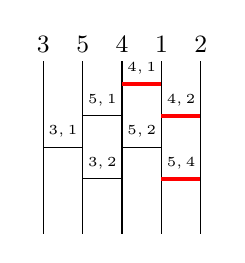
\begin{tikzpicture}
		\draw(0, 0) to (0, 2.2);
			\node at(.25, 1.3){\tiny{$3,1$}};
			\draw(0, 1.1) to (.5, 1.1);
		\draw(.5, 0) to (.5, 2.2);
			\node at(.75, 1.7){\tiny{$5,1$}};
			\draw(.5, 1.5) to (1, 1.5);
			\node at(.75, .9){\tiny{$3,2$}};
			\draw(.5, .7) to (1, .7);
		\draw(1, 0) to (1, 2.2);
			\node at(1.25, 2.1){\tiny{$4,1$}};
			\draw[line width=.5mm, red ](1, 1.9) to (1.5, 1.9);
			\node at(1.25, 1.3){\tiny{$5,2$}};
			\draw(1, 1.1) to(1.5, 1.1);
		\draw(1.5, 0) to (1.5, 2.2);
			\node at(1.75, 1.7){\tiny{$4,2$}};
			\draw[line width=.5mm, red ](1.5, 1.5) to (2, 1.5);
			\node at(1.75, .9){\tiny{$5,4$}};
			\draw[line width=.5mm, red ](1.5, .7) to (2, .7);
		\draw(2, 0) to (2, 2.2);


		\node at(0.0, 2.4){\small{$3$}};
		\node at(0.5, 2.4){\small{$5$}};
		\node at(1.0, 2.4){\small{$4$}};
		\node at(1.5, 2.4){\small{$1$}};
		\node at(2.0, 2.4){\small{$2$}};
	\end{tikzpicture}
	\caption{The route of element 4=(4,1),(4,2),(5,4).}
	\label{Fig:Route}
\end{figure}



The \emph{clean level} is defined as one more than the largest 
element associated with any bar that has undergone a right swap operation. 
For example, if the largest element associated with a bar that has undergone a 
right swap operation is element $4$, then the clean level is $5=4+1$.
 Please refer to Figure~\ref{Fig:CleanLevel} for an example of the clean level.
 If no bars have been right swapped, then the clean level is $1$.
If the largest element to have undergone a right swap operation is the maximal element in $\pi$, 
then the clean level is $max+1$.\pagebreak

\begin{figure}[t]
	\centering 
	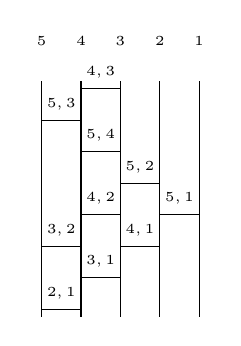
\begin{tikzpicture}
		\draw(0, 0) to (0, 3);
			\node at(.25, 2.7){\tiny{$5,3$}};
			\node at(.25, 1.1){\tiny{$3,2$}};
			\node at(.25, .3){\tiny{$2,1$}};
			\draw(0, 2.5) to (.5, 2.5);			
			\draw(0, .9) to (.5, .9);
			\draw(0, .1) to (.5, .1);

		\draw(.5, 0) to (.5, 3);
			\node at(.75, 3.1){\tiny{$4,3$}};
			\node at(.75, 2.3){\tiny{$5,4$}};
			\node at(.75, 1.5){\tiny{$4,2$}};
			\node at(.75, .7){\tiny{$3,1$}};

			\draw(.5, 2.9) to (1, 2.9);
			\draw(.5, 2.1) to (1, 2.1);
			\draw(.5, 1.3) to (1, 1.3);
			\draw(.5, .5) to (1, .5);
		\draw(1, 0) to (1, 3);
			\node at(1.25, 1.9){\tiny{$5,2$}};
			\node at(1.25, 1.1){\tiny{$4,1$}};

			\draw(1, 1.7) to (1.5, 1.7);
			\draw(1, .9) to (1.5, .9);
		\draw(1.5, 0) to (1.5, 3);
			\node at(1.75, 1.5){\tiny{$5,1$}};
			\draw(1.5, 1.3) to (2, 1.3);
		\draw(2, 0) to (2, 3);

		%%%%%%%%%%%%%%%%%%%%%%%%%%%%
		\node at(0, 3.5){\tiny{$5$}};
		\node at(.5, 3.5){\tiny{$4$}};
		\node at(1, 3.5){\tiny{$3$}};
		\node at(1.5, 3.5){\tiny{$2$}};
		\node at(2, 3.5){\tiny{$1$}};
\end{tikzpicture}
	\caption{A ladder with a clean level of $6$. The largest element whose associated bars have undergone a right swap operation is $5$}
	\label{Fig:CleanLevel}
\end{figure}


Each $OptL\{\pi\}$ has a unique ladder with a clean level of one. This ladder 
is known as the \emph{root ladder}. The root ladder is the root of the tree structure 
produced from {\sc FindAllChildren}. Unlike every other ladder in the tree, 
the root ladder cannot be derived from a local swap operation. Thus, the root ladder 
must be created by another algorithm other than {\sc FindAllChildren}. 
The authors do not provide details on how to create the root ladder. Thus, an 
algorithm for creating the root ladder can be found in the Appendix in Algorithm~\ref{Alg:RootLadder}.
The details of the root ladder are also explained in the Appendix.
Given all permutations of order $n$, the root ladder for the descending permutation requires 
the most rows. 
\begin{theorem}
  The number of rows required for the root ladder of the descending permutation is $2(n-1) - 1$.
\end{theorem}
\begin{proof}
  The number of rows for the ladder data-structure is calculated a follows: When a bar is added to the ladder it can be added 
  to an already existing row or to a new row. 
  If the current state of the ladder is empty then adding the first bar produces the second ladder in
  $L_{n}$. Since the bars are being added bottom right to top left, and the first bar to be added belongs 
  to the $nth$ route, then it must be added to $row=n-1$, $col=n-1$. As bars of the $nth$ route get 
  continuously added to the ladder, each bar is added a row above the previous bar and to a column 
  to the left of the column of the previous bar.
  Since no two bars of the $nth$ route can be on the same row, this will require $n-1$ rows. Note, if they were added to the same 
  row, then the left end point of the right bar would be touching the right end point of the left bar which is disallowed. Once the 
  bars of the $nth$ element are added, the bars of the $n-1th$ route will be added. The $n-1th's$ first bar 
  will be added to the $n-2$ column, otherwise it would be directly below the first bar of the $nth$ route, which is a violation. 
  Since the first bar of the $n-1$'s element is added to column $n-2$, then it must be given a new row, otherwise its right end point 
  will be touching  the left end point of the first bar of route $n$. The remaining $n-2$ bars of element $n-1$
  will be added bottom right to top left, but none of their end points will touch the end points of element $n$ seeing as they will 
  always be two columns apart from any bar in $n's$ route. The same logic applies to element $n-2$, it will require one extra row for its 
  first bar, in order not to touch the first bar of element $n-1$, but the remainder of its bars will always be two columns away from 
  the remainder of the bars for $n-1$, etc. Therefore there are $n-1$ rows required for the $nth$ element and each subsequent 
  element, $k$ requires only one new row. Since $2 \leq k < n$, then there are $(n-2)$ additional rows required for the ladder. Note that element 
  $1$ has no bars in its route. Therefore there are $(n-1)$ rows required for element $n's$ bars  plus $(n-2)$ rows required for 
  all the remaining $2 \leq k < n$ routes. In conclusion the number of rows required is $(n-1) + (n-2) = 2(n-1)-1$. 
  See figure for the tree of ladders 
  generated by {\sc ModifiedSJT} for $n=4$. Note that the maximum number of rows required is $2(n-1)-1=2(3)-1=5$.
\end{proof}



%%Root ladder subsection




%%DONE Appendix SECTION

In concluding the section on the enumeration problem, we have analyzed the original paper along with 
making additions to the algorithm {\sc FindAllChildren} by providing four essential algorithms 
for the completion of {\sc FindAllChildren}. The algorithms are Algorithm~\ref{Alg:RootLadder}, Algorithm~\ref{Alg:RightSwap},
Algorithm~\ref{Alg:LeftSwap} and Algorithm~\ref{Alg:ShiftSubLadder} which can be found in the Appendix. In concert, these five algorithms solve the enumeration 
problem which lists $OptL\{\pi\}$ in $O(1)$ time per ladder. 


\pagebreak


\subsection{Ladder-Lottery Realization}

In their paper \textbf{Ladder-Lottery Realization} the authors provide 
a rather interesting puzzle in regards to ladder lotteries. The puzzle 
is known as the ladder-lottery realization problem. In order to understand
the problem, one must know what a \emph{multi-set} is. A \emph{multi-set}
is a set in which an element appears more than once. The exponent 
above the element indicates the number of times it appears in the set.
For example, given the following multi-set, $\{3^{2}, 2^{4}, 5^{1}\}$ 
the element $3$ appears twice in the set, the element $2$ appears four times
in the set and the element $5$ appears once in the set.
The ladder-lottery realization puzzle asks, given an arbitrary starting permutation 
and a multi-set of bars, 
is there a \emph{non-optimal} ladder lottery for the arbitrary permutation
that uses every bar in the multi-set the number 
of times it appears in the  multi-set. 
For an example of an affirmative solution to the ladder lottery realization problem, see Fig. 2.4.


\begin{figure}[!htp]
    \begin{center}
        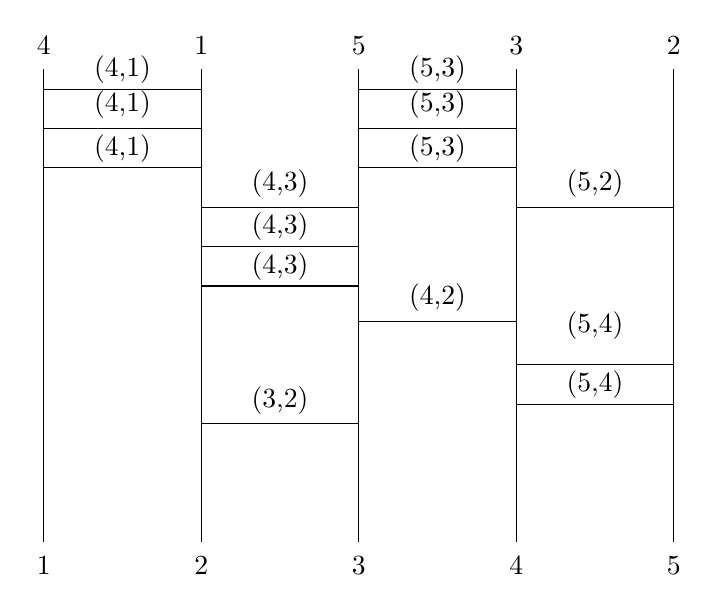
\begin{tikzpicture}
            \draw (0, 0) to (0, 6);
                \node at(0, -0.3){1};
                \node at(0, 6.3){4};
            \draw(2, 0) to (2, 6);
                \node at(2, -0.3){2};
                \node at(2, 6.3){1};
            \draw(4, 0) to (4, 6);
                \node at(4, 6.3){5};
                \node at(4, -0.3){3};
            \draw(6, 0) to (6, 6);
                \node at(6, 6.3){3};
                \node at(6, -0.3){4};
            \draw(8, 0) to (8, 6);
                \node at(8, 6.3){2};
                \node at(8, -0.3){5};

            %%draw the bars
                \node at(1, 6){(4,1)};
                    \draw(0, 5.75) to (2, 5.75);
            \draw(0, 5.25) to (2, 5.25);
                \node at(1, 5.55){(4,1)};
            \draw(0, 4.75) to (2, 4.75);
                \node at(1, 5){(4,1)};

            \draw(4, 5.75) to (6, 5.75);
                \node at(5, 6){(5,3)};
            \draw(4, 5.25) to (6, 5.25);
                \node at(5, 5.55){(5,3)};
            \draw(4, 4.75) to (6, 4.75);
                \node at(5, 5){(5,3)};

            \draw(2, 4.25) to (4, 4.25);
                \node at (3, 4.55){(4,3)};
            \draw(2, 3.75) to (4, 3.75);
                \node at (3, 4){(4,3)};
            \draw(2, 3.25) to (4, 3.25);
                \node at (3, 3.5){(4,3)};
            
            \draw(2, 1.5) to (4, 1.5);
                \node at(3, 1.8){(3,2)};
            
            \draw(4, 2.8) to (6, 2.8);
                \node at (5, 3.1){(4,2)};
            \draw(6, 4.25) to (8, 4.25);
                \node at (7, 4.55){(5,2)};
            
            \draw(6, 2.25) to (8, 2.25);
                \node at (7,2.75){(5,4)};
            
            \draw(6, 1.75) to (8, 1.75);
                \node at (7, 2){(5,4)};
            
        \end{tikzpicture}
    \end{center}
      


    \caption{An affirmative solution to the Ladder Lottery Realization Problem given a starting perumtation $(4,1,5,3,2)$ and the multi set of bars $\{(4,1)^{3}, (4,3)^{3}, (4,2)^{1}, (5,4)^{2}, (5,3)^{3}, (5,2)^{1},(3,2)^{1}\}$}
\end{figure}
\pagebreak
The authors prove that the ladder-lottery realization problem in NP-Hard
by reducing the ladder-lottery realization to the One-In-Three 3SAT, 
which has already been proven to be NP-Hard. The One-In-Three 3SAT 
problem is a problem such that given a set of variables $(X)$, a collection 
of \emph{disjuntcive clauses} $(C)$ which are disjunctive expressions over 
literals of $X$. Each clause in $C$ 
must contain three literals then is there a truth assignment for $X$ such that 
each clause in $C$ has exactly one true literal. For eaxmple, let 
$X=\{p, q, r, s, t\}$ and let $C=\{C_{p,q,s}, C_{r,q,s} C_{p,s,t}, C_{r,t,q}\}$,
the question is whether it is possible for each clause to have exactly one
true literal. The answer in this case is yes. If $p=T$, $r=T$, $q=F$, $s=F$
 and $t=T$ then all the clauses in $C$ have exactly one true literal. 
 The authors reduce the ladder lottery-realization problem to the
One-In-Three 3SAT problem by devising four gadgets. The result of 
the reduction is that the arbitrary starting permutation is equivelent 
to a derivation of the intial set of variables, $X$, in the One-In-Three 3SAT 
problem and the multi-set of bars is equivelent to a 
derivation of the intial set of clauses, $C$, in the One-In-Three 
3SAT problem.\par 
The authors note that there are two cases in which the ladder-lottery
realization problem can be solved in polynomial time. These cases 
include the follwing. First, if every bar in the multi-set appears
exactly once and every bar corresponds to an inversion, 
then an affirmative solution to the ladder-lottery realization 
instance can be demonstrated in polynomial time. 
Second, if there is an inversion in the perumutation and its bar appears in the multi-set an even 
number of times, then a negative solution to
the ladder-lottery realization instance
can be solved in polynomial time.\par
%%%section on how ladde lotteries relate to other mathematical objects
Despite the fact that ladder lotteries have only been stuidied in and
of themseleves for ten years, they are closely tied to other mathematical 
phenomena that have been studied for much longer. These mathematical phenomena  
 include \emph{Pseudo Lines} which are an arrangement of 
curves on a plane such that given two curves, they only intersect 
at most once and at each intersection, only two curves intersect.See figure --reference--
for a wiring diagrams of the pseudo line arrangement for the 
permutation, $(5,4,3,2,1)$. The other mathematical phenomena is \emph{adjacent transpositions}
which is a swap of two adjacent elements in a permutation. 
\subsection{Ladders and Adjacent Transpositions}
A ladder lottery is a way of sorting a permutation, yet it can also be thought of as 
a decomposition of a permutation into \emph{adjacent transpositions}. \cite{A1} 
An \emph{adjacent transposition} is simply a swap of two adjacent elements in a 
permutation. For example, given the permutation (1, 3, 4, 2), an adjacent 
transposition could be done on the following pairs of elements: 
(1, 3), (3, 4) or (4, 2). Each would result in a unique permutation. 
Simply put, given any arbitrary starting permutation, $\pi$, keep swapping 
adjacent inversions until the identity permutation is reached.  An optimal 
ladder lottery from $\pi's$ optimal ladder set is a minimal sequence of 
adjacent transpositions such that $\pi$ is sorted into the identity permutation; 
each ladder in the set represents a sequence of adjacent transpositions for 
sorting $\pi$ into the identity permutation. For example, given the permutation 
(4, 3, 2, 1) there exists eight ladders in this permutation's optimal ladder set. 
Two of these ladders are found in \ref{fig:ac}:

\begin{figure}[!htp]
    \label{fig:ac}
	\begin{minipage}{0.4\textwidth}
		\centering
	
		\begin{tikzpicture}
			\draw(0, 0) to (0, 4) node[above]{4};
			\draw(2, 0) to (2, 4) node[above]{3};
			\draw(4, 0) to (4, 4) node[above]{2};
			\draw(6, 0) to (6, 4) node[above]{1};
			
			\draw(0, 3.7) to (2, 3.7);
				\draw node at (1, 3.9) {(4, 3)};
			\draw(2, 3.25) to (4, 3.25);
				\draw node at (3, 3.45){(4, 2)};
			\draw(4, 2.75) to (6, 2.75);
				\draw node at (5, 3.0){(4, 1)};
			
			\draw(0, 2.75) to (2, 2.75);
				\draw node at (1, 3.0){(3, 2)};
			\draw(2, 2.25) to (4, 2.25);
				\draw node at (3, 2.5){(3, 1)};
			
			
			\draw(0, 1.75) to (2, 1.75);
				\draw node at (1, 1.95){(2, 1)};
			
			\draw node at (0, -0.5){1};
			\draw node at (2, -0.5){2};
			\draw node at (4, -0.5){3};
			\draw node at (6, -0.5){4};
			
			%%second ladder%%
			\draw(9, 0) to (9, 4) node[above]{4};
			\draw(11, 0) to (11, 4)node[above]{3};
			\draw(13, 0) to (13, 4)node[above]{2};
			\draw(15, 0) to (15, 4)node[above]{1};
			
			\draw(9, 3.7) to (11, 3.7);
				\draw node at (10, 3.9) {(4, 3)};
			\draw(11, 3.25) to (13, 3.25);
				\draw node at (12, 3.45){(4, 2)};
			\draw(13, 2.75) to (15, 2.75);
				\draw node at (14, 3.0){(4, 1)};
			
			\draw(9, 1.25) to (11, 1.25);
				\draw node at (10, 1.5){(3, 1)};
			\draw(11, 2) to (13, 2);
				\draw node at (12, 2.25){(2, 1)};
			
			\draw(11, 0.65) to (13, 0.65);
				\draw node at (12, 0.85){(3, 2)};
			 
			
			\draw node at (9, -0.5){1};
			\draw node at (11, -0.5){2};
			\draw node at (13, -0.5){3};
			\draw node at (15, -0.5){4};	
		\end{tikzpicture}
	
	\end{minipage}
	

	
		
	\caption{The left ladder is one of eight unique ladders from (4,3,2,1)'s optimal ladder set. The right ladder is another one of eight unique ladders form (4,3,2,1)'s optimal ladder set}
		
\end{figure}

From looking at the above ladders, going from top left to bottom right, the left ladder represents the sequence of adjacent transpositions (4,3), (4,2), (4,1),(3,2),(3,1),(2,1) 
whereas the right ladder represent the sequence of adjacent transpositions 
(4, 3),(4, 2),(4, 1),(2, 1),(3, 1),(3, 2). 
Notice how the length of the sequences are the same,because both lengths are equal 
to the minimal number of swaps to sort (4, 3, 2, 1) 
it is simply the order in which the adjacent transpositions occur in the sequence 
that makes the sequences different from each other. 